\begin{figure}
    \begin{center}
    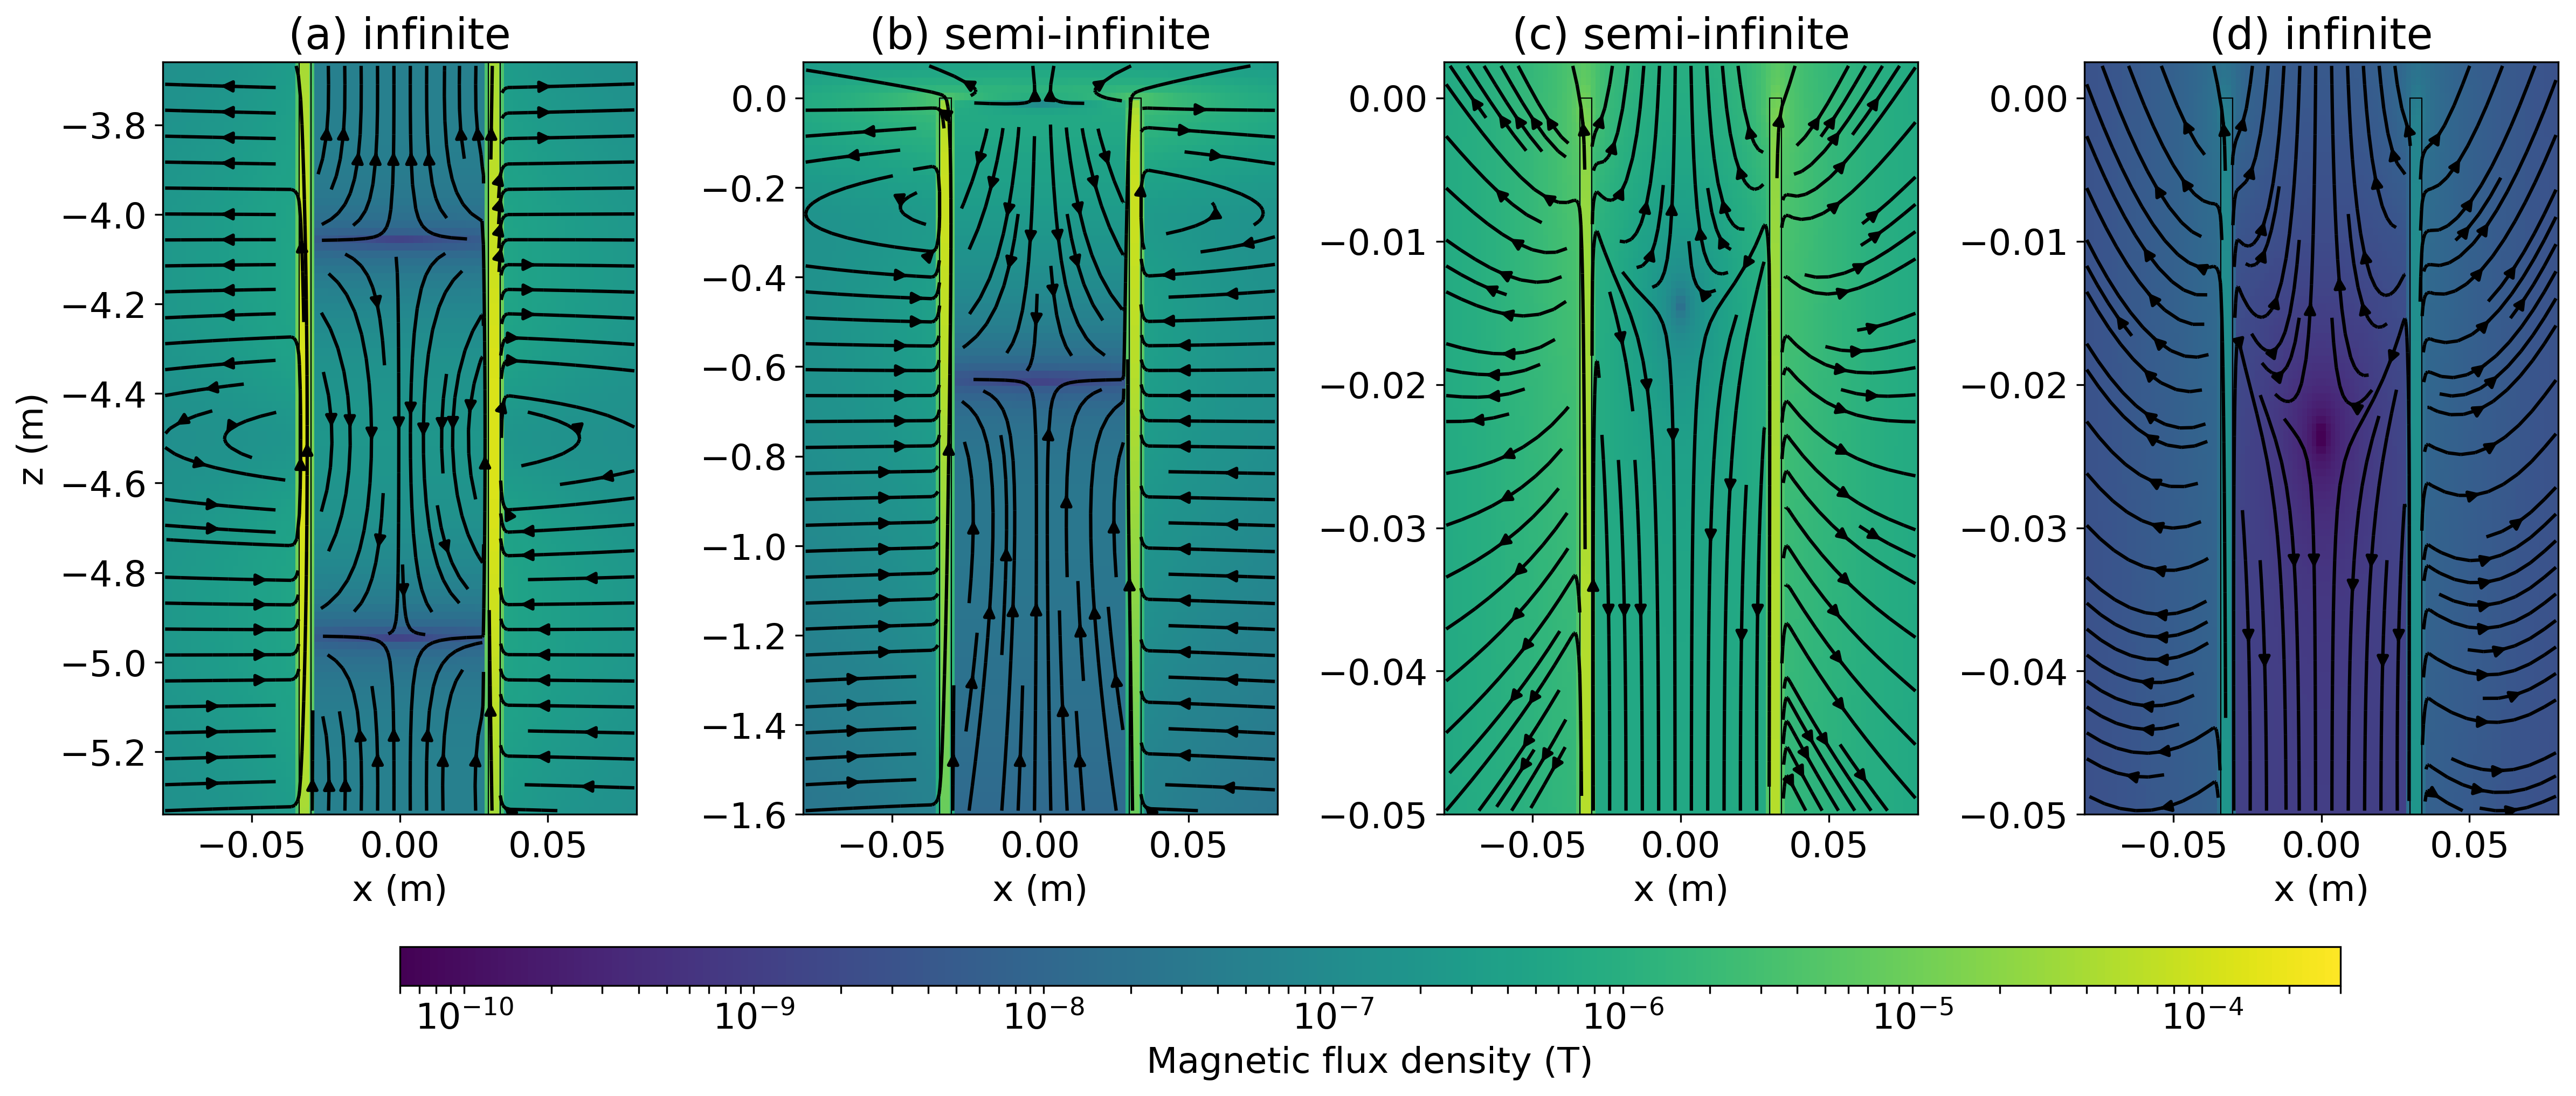
\includegraphics[width=\columnwidth]{figures/casing_software/AugustinBfields.png}
    \end{center}
\caption{
    Magnetic flux density at 0.1 Hz in the region of the pipe near the plane of the source for
    (a) the ``infinite'' pipe, where the source is located at -4.5 m and the pipe extends from 0 m to -9 m,
    (b) a ``semi-infinite'' pipe, where the source is located at 0 m and the pipe extends to -9 m.
    In (c), we zoom in to the top 5 cm of the ``semi-infinite'' pipe,
    and (d) shows the 5 cm at the top-end of the ``infinite'' pipe.
}
\label{fig:AugustinBfields}
\end{figure}
